\documentclass[a4paper]{article}

\usepackage[version=3]{mhchem}
\usepackage{siunitx}
\usepackage{graphicx}
\usepackage{natbib}
\usepackage{amsmath}
\usepackage[utf8]{inputenc}
\usepackage[portuguese]{babel}
\usepackage[left=2cm,right=2cm,top=2cm]{geometry}
\usepackage{multicol}
\usepackage{caption}
\setlength\parindent{0pt}

\renewcommand{\labelenumi}{\alph{enumi}.}
\newcommand{\igo}{\textit{iGo}}

\title{\igo\\Resultados e Análise do Inquérito aos Utilizadores\\\small Interfaces Pessoa Máquina}
\author{Baltasar Dinis 89416, Afonso Ribeiro 86752, Francisco Figueiredo 89443}

\date{\today}
\begin{document}
\maketitle

\begin{abstract}
  Este documento sumariza os resultados do inquérito relativo ao
  wearable iGo. Fazemos ainda a análise dos mesmos, tendo como linhas
  orientadoras as perguntas da Análise de Utilizadores e Tarefas (AUT).
  Finalmente, propomos três funcionalidades a desenvolver, bem como respectivos cenários de utilização.
\end{abstract}

  \section{Resultados Gerais do Inquérito}
  O inquérito foi realizado entre 11 e 15 de Março de 2019 tendo sido recolhido um
  total de 38 respostas.  Os inquiridos foram maioritariamente ($60.5\%$) do sexo
  feminino. A faixa etária mais representada foi a dos $18$ aos $25$ anos ($78.9\%$) dos
  inquiridos, seguida da faixa etária dos $46$ aos $55$ ($7.9\%$).
  A maioria dos inquiridos são estudantes($76.3\%$). As únicas dificuldades físicas
  reportadas foram visuais, onde a Miopia foi a mais indicada ($71.4\%$). A
  maioria dos inquiridos assinalou ter concluído o ensino secundário ($44.7\%$) ou
  ter obtido o grau de licenciado ($42.1\%$).

\begin{multicols}{2}
  \section{Análise de Utilizadores e Tarefas}

  \subsection{Quem vai utilizar o sistema?}
  Com base na amostra, consideramos que os utilizadores serão jovens, com idades
  compreendidas entre os $18$ e os $25$ anos, com um elevado grau de escolaridade.
  O obstáculo mais relevante a endereçar - relativamente a problemas físicos de
  utilizadores - é o de problemas visuais.
  \subsection{Que tarefas executam actualmente?}
  Questionados sobre onde costumam dormir em viagem, $86.8\%$ indicou que pernoita
  em hotéis, $18.4\%$ em parques de campismo e $10.5\%$ em hostéis.
  Relativamente à logística das refeições, concluímos que a grande maioria
  ($81.6\%$) dos utilizadores vai a restaurantes, $60,5\%$ referiu que cozinhava e
  $34.2\%$ afirmou que consume refeições pré feitas.

  \subsection{Que tarefas são desejáveis?}
  Neste tópico foram questionados os tipos de funcionalidades que os utilizadores
  gostariam que o iGo oferecesse. Em resposta, destacaram-se $3$
  ações/recursos que os utilizadores consideram de úteis:
  \begin{tabular}{l  r}
    Mapa com pontos de interesse & $78.9\%$\\
    Navegação GPS & $68.4\%$\\
    Sincronização com dispositivos externos & $68.4\%$\\
  \end{tabular}

  \subsection{Como é que os utilizadores aprendem as tarefas?}
  Aferimos como é que os utilizadores se familiarizam com novas tecnologias, tendo
  chegado à conclusão de que a grande maioria o faz através da experimentação
  ($92.1\%$), mas também com o auxílio de amigos/família($31.6\%$) e de vídeos
  explicativos online ($31.6\%$).
\subsection{Onde são desempenhadas as tarefas?}
Em termos de envolvente humana, os utilizadores reportaram que viajam maioritariamente com a família ($89.5\%$); com amigos
  ($84.2\%$); em grupos de 3-6 pessoas ($78.9\%$). Menos frequentemente, viajam
  em grupos com mais de 5 pessoas ($18.4\%$).

Dada a natureza da rede social e do dispositivo, as tarefas serão desempenhadas
  em atividades turísticas (urbanas ou rurais), ou seja, em terreno
  desconhecido. Isto é coerente com o facto dos utilizadores terem reportado
  necessidade de existir um sistema de navegação GPS e um mapa com pontos de
  interesse.

\subsection{Quais as relações entre utilizadores e informação?}
Relativamente à informação fornecida pelo utilizador ao sistema, $35.1\%$ dão um
  nível 5 (em 5) de importância a partilhar as suas viagens e $51.3\%$ dão uma
  importância entre 3-4. Especificamente sobre a partilha em redes sociais, na
  Figura 1 encontra-se especificado, por elemento da viagem, a importância que
  utilizadores dão a seguinte importância à partilha de vários elementos da
  viagem.
  \begin{center}
    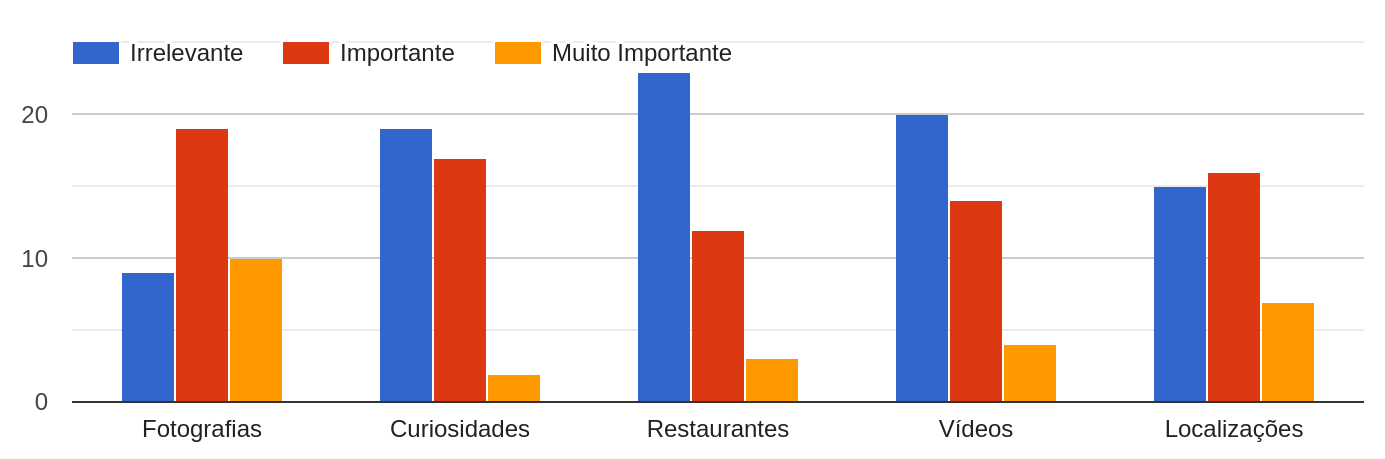
\includegraphics[width=\linewidth]{importance}
    \captionof{figure}{Importância da partilha em redes sociais, por elemento da viagem}
  \end{center}
  Pela análise da Figura 1, concluímos que a partilha de fotografias e
  localizações são os elementos mais importantes.

\subsection{Que outros instrumentos tem o utilizador?}
A maioria dos utilizadores utilizam smartphones e computadores diariamente.
Apenas $10.5\%$ dos utilizadores possuem smartwatch e dos que não têm $47.2\%$
já considerou obter um. Dos que não consideraram obter um smartwatch a maioria
afirma que não sente necessidade/interesse.

\subsection{Como comunicam os utilizadores entre si?}
Foi observado que a maioria dos utilizadores ($94.1\%$) utiliza o smartphone
como meio de comunicação e partilha.

\subsection{Qual a frequência de desempenho das tarefas?}
A maioria dos utilizadores vai de viagem anualmente ($68.4\%$), sendo que
$28.9\%$ indicaram que o fazem mensalmente.
Foi observado que $35.1\%$ das pessoas dão muita importância a partilhar as suas
viagens, sendo que $94.1\%$ das partilhas são feitas através do smartphone.

\subsection{Quais as restrições de tempo impostas?}
O parâmetro avaliados nesta questão foi o tempo que os utilizadores estariam
dispostos a esperar para efetuar variadas tarefas no iGo. Através da análise das
respostas, concluímos que as pessoas querem conseguir partilhar fotografias, vídeos e
abrir o mapa e localizar-se no mesmo quase instantaneamente ($10s$). Para procurar restaurantes na área e
receber estatísticas dos sinais fisiológicos já estão dispostos a receber
respostas rápidas ($30s$). Em procurar estadia e pontos de interesse obtiveram-se
percentagens de respostas semelhantes para tempos quase instantâneos e rápidos.
\subsection{}
Os utilizadores foram inquiridos relativamente a como reagem a falhas nos
instrumentos eletrónicos. Obtivemos as seguintes respostas:
\begin{itemize}
  \item $55.3\%$ recorrem ao suporte técnico
  \item $52.6\%$ tentam resolver sozinhas
  \item $42.1\%$ pedem ajuda a amigos/conhecidos
  \item $31.6\%$ procuram online por vídeos explicativos
\end{itemize}
Note-se que nenhum utilizador indicou que abandonaria o dispositivo.
\end{multicols}

\section{Funcionalidades}
Os utilizadores votaram nas funcionalidades propostas no questionário da
seguinte forma:

\begin{center}
  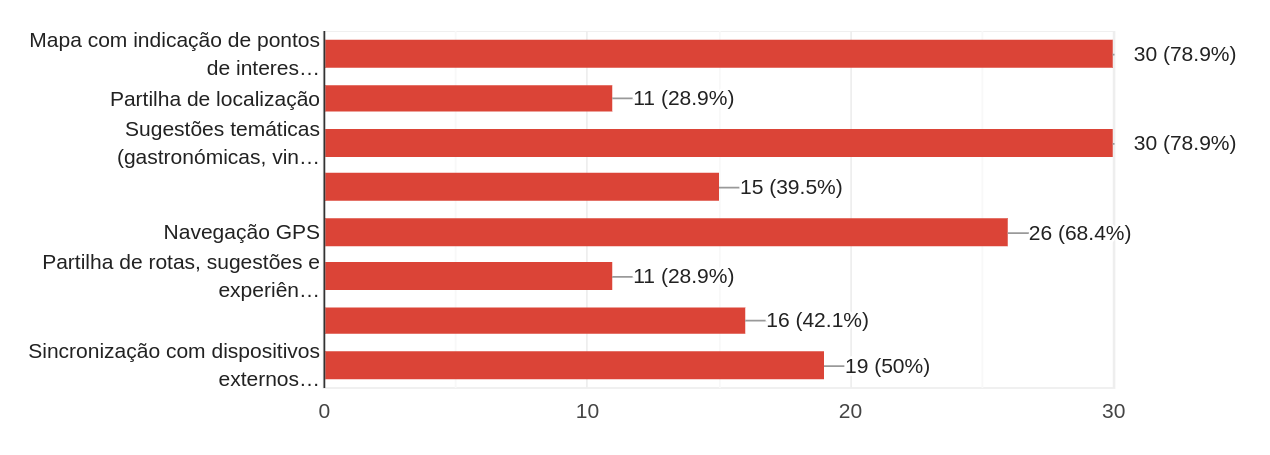
\includegraphics[width=\linewidth]{resp}
  \captionof{figure}{Importância da partilha em redes sociais, por elemento da viagem}
\end{center}
\begin{multicols}{2}

  \subsection{Mapa navegável com indicação dos pontos de interesse}
  Neste mapa, que oferece navegação, os utilizadores estão centrados no mesmo e
  os pontos de interesse estão assinalados. É possível escolher os tipos de
  pontos a mostrar no mapa.

  \textbf{Caso de Utilização:} O João - com 49 anos e empregado - quer visitar
  um museu perto de si. Para tal, utiliza o seu wearable \igo . No dispositivo,
  consegue filtrar os pontos de interesse para que e

  \subsection{Sincronizar com dispositivos externos de captura de vídeo}
  Os utilizadores podem remotamente mas com próximidade relativa do dispositivo
  externo de observar no wearable o que é captado pelo dispositivo de captura de
  vídeo.

  \textbf{Caso de Utilização:} A Inês encontrasse na sua viagem anual com o seu
  grupo de 7 amigos e pretende usar o seu drone para fazer um vídeo
  aéreo do seu grupo. Emparelha o drone com o seu dispositivo \igo, e, com o
  drone no ar, consegue confirmar no \igo  o enquadramento da fotografia, antes
  de a tirar.

  \subsection{Partilha de fotografias}
  Os utilizadores podem partilhar fotografias para as redes sociais

  \textbf{Caso de Utilização:} A Joana - de 21 anos e aluna de terceiro ano da
  faculdade - acabou de tirar uma fotografia e quer
  partilha-la na sua rede social favorita - o MyWeb. Vai às fotografias no seu
  dispositivo \igo  e escolhe a última fotografia que tirou e partilha-a.

\end{multicols}

\end{document}
